\documentclass[12pt,a4paper]{scrartcl} 
\usepackage[utf8]{inputenc}
\usepackage[english,russian]{babel}
\usepackage{indentfirst}
\usepackage{misccorr}
\usepackage{graphicx}
\usepackage{indentfirst}
\usepackage{amsmath}
\usepackage{mathtools}
\usepackage{fancyhdr}
\usepackage{minted}
\setminted{
    style=emacs,
    breaklines=true,
    autogobble=true,
    linenos=true,
    frame=single,
    fontsize=\small
}

\begin{document}
 \begin{titlepage}
  \begin{center}
   \large
   МИНИСТЕРСТВО НАУКИ И ВЫСШЕГО ОБРАЗОВАНИЯ РОССИЙСКОЙ ФЕДЕРАЦИИ
   
   Федеральное государственное бюджетное образовательное учреждение высшего образования
   
   \textbf{АДЫГЕЙСКИЙ ГОСУДАРСТВЕННЫЙ УНИВЕРСИТЕТ}
   \vspace{0.25cm}
   
   Инженерно-физический факультет
   
   Кафедра автоматизированных систем обработки информации и управления
   \vfill

   \vfill
   
   \textsc{Отчет по практике}\\[2mm]
   
   {\LARGE Создать программу для генерации случайных паролей заданной длины и сложности
    \vspace{0.25cm}
   
   \textit{Вариант 1}}
   \bigskip
   
   2 курс, группа 2ИВТ1-1
  \end{center}
  \vfill
  
  \newlength{\ML}
  \settowidth{\ML}{«\underline{\hspace{0.7cm}}» \underline{\hspace{2cm}}}
  \hfill\begin{minipage}{0.5\textwidth}
   Выполнил:\\
   \underline{\hspace{\ML}} Д.\,А.~Лиев\\
   «\underline{\hspace{0.7cm}}» \underline{\hspace{2cm}} 2024 г.
  \end{minipage}%
  \bigskip
  
  \hfill\begin{minipage}{0.5\textwidth}
   Руководитель:\\
   \underline{\hspace{\ML}} С.\,В.~Теплоухов\\
   «\underline{\hspace{0.7cm}}» \underline{\hspace{2cm}} 2024 г.
  \end{minipage}%
  \vfill
  
  \begin{center}
   Майкоп, 2024 г.
  \end{center}
 \end{titlepage}
 
% Содержание
\section{Введение}
\label{sec:intro}


\subsection{Формулировка цели}
Целью данной работы является написание программы для генерации случайных паролей заданной длины и сложности.

\subsubsection{Теория}
Генерация случайных паролей важна для обеспечения безопасности данных. Сильный пароль должен обладать следующими характеристиками. Во-первых, достаточная длина: чем длиннее пароль, тем сложнее его взломать методом перебора. Во-вторых, сложность: использование различных типов символов (буквы, цифры, специальные символы) увеличивает количество возможных комбинаций и затрудняет взлом.

Основные требования к случайным паролям:
    \begin{enumerate}
        \item пароли должны генерироваться случайным образом, чтобы предотвратить предсказуемость;
        \item для повышения стойкости должны использоваться различные символы;
        \item пользователь должен иметь возможность задать параметры генерации, такие как длина и сложность пароля.
    \end{enumerate}
    \noindent 

Для генерации случайных паролей используются псевдослучайные генераторы чисел (PRNG). В C++ доступны стандартные библиотеки для работы с случайными числами и строками, которые можно использовать для этой задачи.

\subsubsection{Практика}
Рассмотрим шаги по созданию программы для генерации случайных паролей на C++:
\begin{enumerate}
        \item пользователь должен иметь возможность задать длину пароля и выбрать уровень сложности, включая использование цифр, специальных символов, заглавных и строчных букв;
        \item используются стандартные библиотеки <random> для генерации случайных чисел. Создается набор символов в зависимости от выбранного уровня сложности. Генерируется случайная последовательность символов заданной длины;
        \item  программа реализована на языке C++ с использованием консольного ввода/вывода;
        \item проведено тестирование для проверки корректности генерации паролей разной длины и сложности. Также проверена непредсказуемость и отсутствие повторяемости паролей.
    \end{enumerate}
    \noindent 

Важно отметить, что программа предоставляет пользователю гибкие настройки для генерации паролей, включая выбор длины и набора используемых символов. Это позволяет создавать пароли разного уровня сложности, удовлетворяющие требованиям безопасности.

В результате проделанной работы была создана программа для генерации случайных паролей на языке C++, отвечающая заданным требованиям по длине и сложности. Программа успешно прошла тестирование и может быть использована для создания безопасных паролей. В будущем возможно расширение функционала программы, включая графический интерфейс и дополнительные параметры настройки паролей.


\section{Ход работы}
\subsection{Программа}
Код выполненной программы:
\begin{minted}[caption={Python code}]{python}
#include <iostream>
#include <string>
#include <random>
#include <ctime>

using namespace std;

string generatePassword(int length, bool useDigits, bool useSpecial, bool useUpper, bool useLower) {
	const string digits = "0123456789";
	const string special = "!@#$%^&*()-_=+[]{}|;:'\",.<>?/\\";
	const string upper = "ABCDEFGHIJKLMNOPQRSTUVWXYZ";
	const string lower = "abcdefghijklmnopqrstuvwxyz";

	string characterPool;

	if (useDigits) characterPool += digits;
	if (useSpecial) characterPool += special;
	if (useUpper) characterPool += upper;
	if (useLower) characterPool += lower;

	if (characterPool.empty()) {
		throw invalid_argument("Необходимо выбрать хотя бы один тип символов для генерации пароля.");
	}

	string password;
	mt19937 generator(static_cast<unsigned>(time(nullptr)));
	uniform_int_distribution<> distribution(0, characterPool.size() - 1);

	for (int i = 0; i < length; ++i) {
		password += characterPool[distribution(generator)];
	}

	return password;
}

int main() {
	setlocale(LC_ALL, "Rus");
	system("chcp 1251");

	int length;
	string input;

	cout << "Введите длину пароля: ";
	cin >> length;

	cout << "Использовать цифры? (да/нет): ";
	cin >> input;
	bool useDigits = (input == "да");

	cout << "Использовать специальные символы? (да/нет): ";
	cin >> input;
	bool useSpecial = (input == "да");

	cout << "Использовать заглавные буквы? (да/нет): ";
	cin >> input;
	bool useUpper = (input == "да");

	cout << "Использовать строчные буквы? (да/нет): ";
	cin >> input;
	bool useLower = (input == "да");

	try {
		string password = generatePassword(length, useDigits, useSpecial, useUpper, useLower);
		cout << "Сгенерированный пароль: " << password << endl;
	}
	catch (const invalid_argument & e) {
		cerr << e.what() << endl;
	}

	return 0;
}
\end{minted}

\subsection{Результат работы программы}
Программа работает следующим образом:

\begin{enumerate}
    \item пользователь вводит длину пароля;
    \item пользователь указывает, будет ли использоваться каждый из следующих типов символов: цифры, специальные символы, заглавные буквы, строчные буквы;
    \item программа генерирует пароль, используя выбранные типы символов.
    \end{enumerate}
    \noindent

Результат работы программы (Рис. 1.):

\begin{figure}[h]
 \centering
 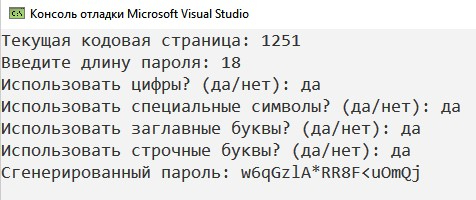
\includegraphics[width=0.62\textwidth]{1.jpg}
 \caption{Результат работы программы}\label{fig:par}
\end{figure}

\begin{thebibliography}{9}
\bibitem{Knuth-2003}Кнут Д.Э. Всё про \TeX. \newblock --- Москва: Изд. Вильямс, 2003 г. 550~с.
\bibitem{Lvovsky-2003}Львовский С.М. Набор и верстка в системе \LaTeX{}. \newblock --- 3-е издание, исправленное и дополненное, 2003 г.
\bibitem{Voroncov-2005}Воронцов К.В. \LaTeX{} в примерах. 2005 г.
\end{thebibliography}

\end{document}